\section{Structured Assurance Case Metamodel and the Goal Structuring Notation}
SACM is designed to support existing safety notations such as GSN and CAE. In previous sections, we briefly demonstrated the semantics of SACM elements by comparing them with GSN notations. In this section, we provide a GSN metamodel that is compliant to SACM. 

\subsection{The GSN Metamodel}
As previously discussed, SACM provides a richer set of features comparing to GSN, which includes the ability to standardise evidential and informational artifacts in the models, standardising controlled grammar and terminologies, as well as modular organisation and integration of artifacts and terminologies. In general, creating a metamodel for GSN is a simple task, for there are only several concepts that GSN captures. However, we think it is more ideal to create the GSN metamodel by extending SACM elements, so that not only the GSN metamodel can inherit features naturally provided by SACM, but also making the interoperability from GSN to SACM easier. 
\begin{figure}
	\centering
	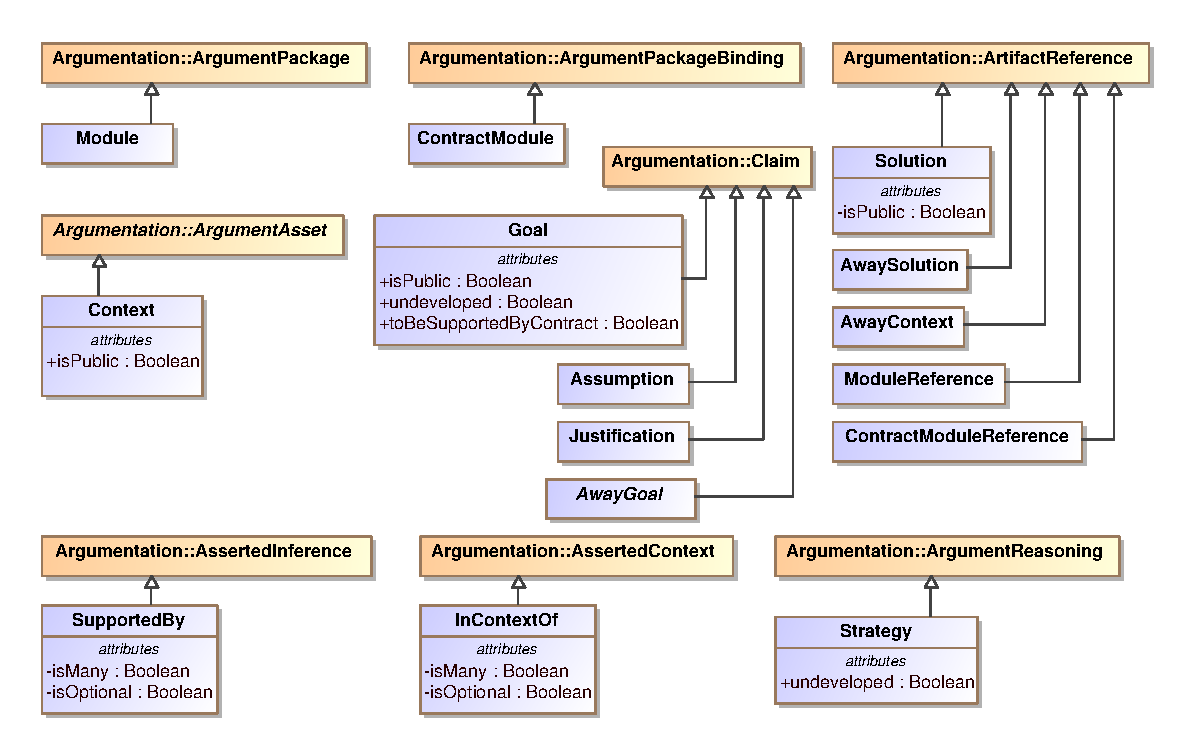
\includegraphics[width=1\linewidth]{GSN.eps}
	\caption{SACM compliant GSN metamodel.}
	\label{fig:gsnMetamodel}
\end{figure}

Our version of the GSN metamodel is shown in Figure~\ref{fig:gsnMetamodel}. In GSN, argumentations are organised in \textit{Module}s, which is made as a sub-type of \textit{ArgumentPackage} in SACM; \textit{ContractMoudle} are essentially contracts that binds \textit{Module}s together, thus it is a sub-type of \textit{ArgumentPackageBinding}. 

Elements \textit{Goal}, \textit{Assumption}, \textit{Justification} and \textit{AwayGoal} are made sub-types of \textit{Claim} in SACM. A \textit{Goal} can be \textit{uninstantiated}, which basically means it is abstract, this is captured by the \textit{+isAbstract} feature in SACM's \textit{SACMElement} class. A \textit{Goal} can be \textit{public}, which is deprecated in SACM, a \textit{Goal} can also be \textit{undeveloped} and \textit{toBeSupportedByContract}, which are captured individually. 

Elements \textit{Solution}, \textit{AwaySolution}, \textit{AwayContext}, \textit{ModuleReference} and \textit{ContractModuleReference} are sub-types of \textit{ArtifactReference} in SACM as they refer to artefacts that contain information they represent. \textit{Context} is a slightly complicated concept, as it can either be a statement stating the context of a \textit{Claim}, or it can refer to contextual information stored in an artefact. Thus, \textit{Context} is made a sub-type of \textit{ArgumentAsset}. 

\textit{SupportedBy} is made a sub-type of \textit{AssertedInference} and \textit{InContextOf} is made a sub-type of \textit{AssertedContext}. \textit{Strategy} is made a sub-type of \textit{ArgumentReasoning} for it explains the intention of an \textit{AssertedRelationship}.

The way that the GSN metamodel is created makes it inherently capable of modelling artefacts and terminologies due to the fact that the GSN metamodel also inherits the the \textit{Base}, \textit{AssuranceCase}, \textit{Artifact} and \textit{Terminology} packages. Our vision is that such GSN metamodel is able to create goal structures, and link evidential and contextual information from the goal structures to their supporting materials, modelling using the \textit{Artifact} and \textit{Terminology} packages. 

\subsection{GSN to SACM Transformation}

\begin{algorithm}[ht!]
	{
		\fontsize{9}{10}
		\selectfont
		\SetAlgoLined\DontPrintSemicolon
		\SetKwFunction{startElement}{startElement}
		\SetKwFunction{endElement}{endElement}
		\SetKwFunction{createModelElement}{createModelElement}
		\SetKwFunction{getCachedModelElement}{getCachedModelElement}
		\SetKwFunction{setFeatureValue}{setFeatureValue}
		\SetKwFunction{setAttributeValue}{setAttributeValue}
		\SetKwFunction{handleObjectAttributes}{handleObjectAttributes}
		\SetKwFunction{handleFeature}{handleFeature}
		
		\SetKwFunction{shouldHandleFeature}{shouldHandleFeature}
		
		\SetKwProg{Procedure}{Procedure}{}{}
		
		\Let stack = new stack of model elements;\\
		\Let cache = new set of model elements;\\
		\Let model = new model;\\
		\Let elements = new stack of xml elements;\\
		\Let EM = the defined/extracted effective metamodel;\\
		\Let referencesToHandle = non-containment references to resolve after file is
		fully read;\\
		
		\Procedure{\startElement{xmlElement}}{
			push xmlElement to elements;\\
			\Let peekModelElement = peek top model element of stack;\\
			\If {peekModelElement is nil} {
				// We are at a root element\\
				\Let type = find a model element type for the tag name of the xmlElement;\\
				\Let modelElement = createModelElement(type);\\
				push modelElement to the stack;\\
			}
			\Else {
				\Let peekModelElementType = the type of \emph{peekModelElement};\\
				\If{a feature needs to be created based on peekModelElementType and
					xmlElement} {
					handleFeature(xmlElement);\\
				}
				
				\ElseIf{a (top level) model element to be created}{
					\Let type = find a model element type for the tag name of the xmlElement;\\
					\Let modelElement = createModelElement(type);\\
					push modelElement to the stack;
				}
			}
		}
		
		\Procedure{\endElement{element}} {
			pop the top model element from the stack;\\
			pop the top model element from the elements;\\
		}
	}
	\
	\caption{Partial Loading Algorithm 1 of 3}
	\label{partial-loading-algo-part1}
\end{algorithm}